

% \documentclass[10pt,journal,onecolumn ]{IEEEtran}
 % \documentclass[final,letter ]{IEEEtran}
% \documentclass[10pt,twocolumn ]{IEEEtran}
%
 \documentclass[10pt,onecolumn,twoside,letter]{IEEEtran}

% If IEEEtran.cls has not been installed into the LaTeX system files,
% manually specify the path to it like:
% \documentclass[12pt,journal,compsoc]{../sty/IEEEtran}

\usepackage{url}
%\usepackage{natbib}
\usepackage{amsmath}
\usepackage{amsfonts}
\usepackage{theorem}
\usepackage[dvips]{epsfig}      % ******* for figures ***************
\usepackage{graphicx}
\usepackage{enumerate}

\usepackage{verbatim}
\usepackage{amssymb}
\usepackage{amsbsy}
\usepackage{setspace}
\usepackage{url}

\theoremstyle{plain}
\newtheorem{Theorem}{Theorem}
\newtheorem{Lemma}{Lemma}
\newtheorem{Proposition}{Proposition}
\newtheorem{Corollary}{Corollary}
\newtheorem{Conjecture}{Conjecture}
\newtheorem{Problem}{Problem}

 \newcommand{\Ave}{\operatorname{Ave}}
 \newcommand{\Int}{\operatorname{Int}}
 \newcommand{\real}{\operatorname{Re}}

{\theorembodyfont{\rmfamily} \newtheorem{Remark}{Remark}}
{\theorembodyfont{\rmfamily} \newtheorem{Assumption}{Assumption}}
{\theorembodyfont{\rmfamily} \newtheorem{Example}{Example}}
{\theorembodyfont{\rmfamily} \newtheorem{Definition}{Definition}}
{\theorembodyfont{\rmfamily} \newtheorem{Question}{Question}}

\newcommand {\R}{\mathbb R}
\newcommand {\A}{\mathbb A}

\newcommand{\be}{\begin{equation}}
\newcommand{\ee}{\end{equation}}
\newcommand{\sgn}{\operatorname{{\mathrm sgn}}}
%%%%%%%%\newcommand{\ve}[1]{\mbox{\boldmath${#1}$}}
\newcommand{\V}{\mathcal V}
\newcommand{\U}{\mathcal U}
\newcommand{\N}{\mathbb N_0}
\newcommand{\B}{\mathcal B \mathcal B}
\newcommand{\W}{\mathcal W}

\newcommand{\sname}{} \newcommand{\slabel}[1]{\debug{\fbox{\tiny \sname #1}}\label{\sname #1}}
\newcommand{\debug}[1]{}              % final version
\newcommand{\FB}{\begin{figure}[t]\centering} \newcommand{\FE}[2]{\caption{#2 \debug{\fbox{\sname #1}}} \slabel{#1} \end{figure}} \newcommand{\tB}{\begin{table}[hbtp]\centering}
\newcommand{\tE}[2]{\caption{#2 \debug{\fbox{\sname #1}}}\slabel{#1} \end{table}} \newcommand{\FIG}[3]{\FB\finput{#1}\FE{#2}{#3}}
\newcommand{\finput}[1]{\input{#1}}   % input figures
%%%% Example: \FIG{fig1}{1-fig}{The Multilink environment}

% counter used by the single column equation
\newcounter{mytempeqncnt}

% correct bad hyphenation here
%\hyphenation{op-tical net-works semi-conduc-tor}


\begin{document}
%
 \title{Synchronization of Coupled Pendulums\thanks{This research is partially supported by a   research grant
from  the  Israeli Ministry of ....}}


%%\begin{comment}
%%%%%%%%
\author{Elad Venezian  and Michael Margaliot \IEEEcompsocitemizethanks{\IEEEcompsocthanksitem
E. Venezian is with the School of Electrical Engineering, Tel-Aviv
University, Tel-Aviv 69978, Israel.
E-mail: ravehalon@gmail.com \protect\\
M. Margaliot is with the School of Electrical Engineering and the Sagol School of Neuroscience, Tel-Aviv
University, Tel-Aviv 69978, Israel.
E-mail: michaelm@eng.tau.ac.il \protect\\
}}
%\end{comment}


\maketitle


\begin{abstract}
%%%%

%%%%
 %%
\end{abstract}

\begin{IEEEkeywords}
%%

%%%
\end{IEEEkeywords}




%% Introduction
%%%%%%%%%
\section{Introduction}
%%%%%%%%%%%%%%%%%%%%%%%%%%%%%%%%%%%




\section{The  model}\label{sec:model}
%%%%%%%%%%%%%%%
Consider a nonlinear pendulum with forcing~$u$:
\[
            \ddot x+\alpha \dot  x+\sin(x)=u ,
\]
where~$x$ is the angle, and~$\alpha>0$.

Define~$\dot{y}:=-\frac{\alpha}{2}\dot{x} -sin(x)+u(t)$. Then
\[
            \ddot x =\dot y-\frac{\alpha}{2}\dot{x}   
\]
\[
          \dot x = y-\frac{\alpha}{2}x
\]
\[
          \dot y =-sin(x)-\frac{\alpha}{2}y+\frac{\alpha^2}{4}x + u(t)
\]
  Thus,
\begin{align*}
%%%
                \begin{bmatrix} \dot x \\ \dot y \end{bmatrix} = \begin{bmatrix} -\frac{\alpha}{2}x+y \\  \frac{\alpha^2}{4}x-\sin(x)-\frac{\alpha}{2} y \end{bmatrix}
                +\begin{bmatrix} 0 \\u \end{bmatrix}.
%%%
\end{align*}
The Jacobian of this dynamics is
\[
            J=\begin{bmatrix}   -\frac{\alpha}{ 2} & 1 \\\frac{\alpha^2}{4}-\cos(x) &-\frac{\alpha}{2}       
               \end{bmatrix},
\]
and its symmetric part is 
\[
            J_s:=\frac{J+J'}{2}= \begin{bmatrix}   -\frac{\alpha}{ 2} & \frac{  1-\cos(x)+\frac{\alpha^2}{4}}{2}\\
           \frac{  1-\cos(x)+\frac{\alpha^2}{4}}{2} &-\frac{\alpha}{2}
               \end{bmatrix}.
\]
%%%%%%%%%%%%%%%%%%%%%%%%%%%%%%%%%%%%%%%%%%
%%%%%%%%%%%%%%%%%%%%%%%%%%%%%%%%%%%%%%%%%
The eigenvalues of~$J_s$ are
\[
             \frac{1}{2} \left(  -  {\alpha}  \pm   |  1-\cos(x)+\frac{\alpha^2}{4}  | \right)=\frac{1}{2} \left(  -  {\alpha}  \pm    (  1-\cos(x)+\frac{\alpha^2}{4} )   \right),
\]
so
\[
            \lambda_{\max}(J_s)=\frac{1}{2} \left(   (\frac{\alpha}{2}-1)^2 -\cos(x)     \right).
\]
Let~$q \in[0,\pi/2]$ satisfy~$\cos(q)=(\frac{\alpha}{2}-1)^2$.
(THIS MEANS THAT WE NEED ABOUND ON ALPHA, NO?)
Then~$ \lambda_{\max}(J_s)<0$ for all~$x\in(-q,q)$.
In particular, for~$\alpha=2$, we have that~$ \lambda_{\max}(J_s)<0$ for all~$x\in(-\pi/2,\pi/2)$.

 
Recall that for the Euclidean vector norm, the induced
matrix norm is~$|A|=(\lambda_{\max}(A'A))^{1/2} $,
 and the induced matrix measure is~$\mu(A)=\lambda_{\max}( \frac{A+A'}{2} )$ (see, e.g.,~\cite{vid}).
Standard arguments from contraction theory (see, e.g.,~\cite{LOHMILLER1998683,sontag_contraction_tutorial}) imply
that   trajectories that remain in the closed  region~$x \in [-q-\varepsilon,q+\varepsilon]$, with~$\varepsilon>0$,
contract with respect to the Euclidean  vector  norm. 

\section{Two cuppeld pendelums}\label{sec:cuppeldPendelums}

According to theorem 3 at \cite{PARTIL_CONTRACTION_SLOTINE}), if two dynamics equations of two coupled systems verify: $\dot{x_1}-h(x_1) = \dot{x_2}-h(x_2)$, where the function $h$ id contracting, then $x_1$ and $x_2$ will converge to each other exponentially, regardless of the initial conditions. We will show that two coupled pendulums verify these conditions:
\\
\\
Let us a consider two nonlinear pendulums which coupled by linear coupling:
\[
            \ddot{x_1}+\alpha \dot{x_1}+\sin(x_1)=D(\dot{x_2}-\dot{x_1})+K(x_2-x_1) ,
\]
\[
            \ddot{x_2}+\alpha \dot{x_2}+\sin(x_2)=D(\dot{x_1}-\dot{x_2})+K(x_1-x_2) ,
\]
\[
            \ddot{x_1}+(\alpha+D) \dot{x_1}+\sin(x_1)+Kx_1 -D\dot{x_2}-Kx_2=\ddot{x_2}+(\alpha+D) \dot{x_2}+\sin(x_2)+Kx_2 -D\dot{x_1}-Kx_1 ,
\]
\[
            \ddot{x_1}+(\alpha+2D) \dot{x_1}+\sin(x_1)+2Kx_1=\ddot{x_2}+(\alpha+2D) \dot{x_2}+\sin(x_2)+2Kx_2 ,
\]
Now, lets define:
\[
     \dot{y_1}:=-2K x_1 -\sin(x_1) -\frac{\alpha+2D}{2}\dot{x_1}, \ \ \ \ \dot{y_2}:=-2K x_2 -\sin(x_2) -\frac{\alpha+2D}{2}\dot{x_2}
\]
\[
            \ddot{x_1}-\dot{y_1}+\frac{\alpha+2D}{2}\dot{x_1}=\ddot{x_2}-\dot{y_2}+\frac{\alpha+2D}{2}\dot{x_2} ,
\]
\[
            \dot{x_1}-\dot{x_2} =y_1-\frac{\alpha+2D}{2}x_1-(y_2-\frac{\alpha+2D}{2}x_2),
\]
\[
     \dot{y_1}-\dot{y_2}:=-2K x_1 -\sin(x_1) -\frac{\alpha+2D}{2}(\dot{x_1}-\dot{x_2})+2K x_2+\sin(x_2)
\]
\[
\dot{y_1}-\dot{y_2}=-2K x_1- \sin(x_1)-\frac{\alpha+2D}{2}y_1+\frac{\alpha+2D}{2} y_2+ \frac{(\alpha+2D)^2}{4} x_1-\frac{(\alpha+2D)^2}{4} x_2+2K x_2+\sin(x_2)
\]
Lets define 

\[\underline{z} =  \begin{bmatrix} x \\ y \end{bmatrix},\ \ \ \ \ \underline{f}(\underline{z}) = \begin{bmatrix} y_1-\frac{\alpha+2D}{2}x_1 \\ -2K x_1- \sin(x_1)-\frac{\alpha+2D}{2}y_1+ \frac{(\alpha+2D)^2}{4} x_1 \end{bmatrix}
\]
And now: 
\[\underline{z_1}-\underline{z_2}=\underline{f}(\underline{z_1})-\underline{f}(\underline{z_2})
\]
And according the theorem: 
\[|\underline{z_2}(t)-\underline{z_1}(t)| <=e^{\lambda_{max}}|\underline{z_2}(0)-\underline{z_1}(0)|
\]
Where \[\lambda_{max}:=\sup_{t>=0} max(max(\lambda(J_s(\underline{z_1}(t))),max(\lambda(J_s(\underline{z_2}(t))))=\sup_{t>=0} max(max(\lambda(J_s(x_1(t))),max(\lambda(J_s(x_2(t))))
\]

Let us show explicitly the value of $\underline{z}(x,\dot x)$:
\[\underline{z} =  \begin{bmatrix} x \\ y \end{bmatrix}, \ \ \ \ \ \   \dot{y}=-2K x -\sin(x) -\frac{\alpha+2D}{2}\dot{x}, \ \ \ \ \ \ y = - \int\limits_0^t
(2K x +\sin(x))dt-\frac{\alpha+2D}{2}x+const
\]
And we will calculate the constant from the initial conditions:
\[ \dot{x} = y-\frac{\alpha+2D}{2}x,
\]
\[ y(0) = \dot{x}(0)+\frac{\alpha+2D}{2}x(0) = -\frac{\alpha+2D}{2}x(0)+const,
\]
\[ \dot{x} = y-\frac{\alpha+2D}{2}x,
\]
\[ const = \dot{x}(0)+(\alpha+2D)x(0),
\]
\section{Angular Velocity Coupling}\label{sec:AngularVelocityCoupling}
For coupling of angular velocity there exist coupling factor $D$, and the phase coupling factor $K=0$. In this case, we will get $\underline{f}$ which is same to the function we got at section 1, but instead the given $\alpha$ we will have the term $\alpha+2D$.

\section{Angular Velocity and Phase Coupling}\label{sec:AngularVelocityAndPhaseCoupling}
For coupling of angular velocity and phase, we will have both $D$ and $K$. So we should check that 
\[
\underline{f}(\underline{z}) = \begin{bmatrix} -\frac{\alpha+2D}{2}x+y \\  \frac{(\alpha+2D)^2}{4}x-\sin(x)-2K-\frac{\alpha+2D}{2} y \end{bmatrix}
\]
is contracting.
\[
            J= \begin{bmatrix}   
 -\frac{\alpha+2D}{ 2} & 1 \\
 \frac{(\alpha+2D)^2}{4}-\cos(x)-2K & -\frac{\alpha+2D}{2}       
               \end{bmatrix},
\]
and its symmetric part is 
\[
            J_s= \begin{bmatrix}  -\frac{\alpha+2D}{ 2} & \frac{  1-\cos(x)+\frac{(\alpha+2D)^2}{4} -2K}{2}\\
           \frac{  1-\cos(x)+\frac{(\alpha+2D)^2}{4} -2K}{2} &-\frac{\alpha+2D}{2}
               \end{bmatrix}.
\]
The eigenvalues of~$J_s$ are
\[
             \frac{1}{2} \left(  -  {\alpha}  \pm   |  1-\cos(x)+\frac{\alpha^2}{4} -2K | \right)=\frac{1}{2} \left(  -  {\alpha}  \pm    (  1-\cos(x)+\frac{\alpha^2}{4} -2K)   \right),
\]
Now, these values are same to the eigenvalues which we get at section 2, except the $\pm K$ term. This factor can "balance" the two eigenvalues, and with wise $K$, it is possible to increase both the region of contraction, and the contraction rate. 

\section{Simulation}\label{sec:Simulation}
We made a simulation where $\alpha+2D = 4,  K = 5$. The initial conditions $x_1, x_2, \dot x_1,\dot x_2$ were selected randomly.

\begin{figure}
\begin{centering}
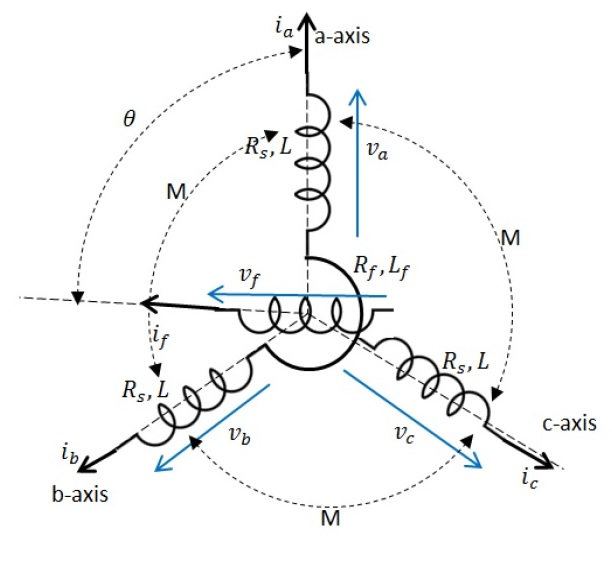
\includegraphics[scale=0.65]{FIG1} 
\par\end{centering}
\caption{\label{fig:Struct}Structure of an idealized three-phase
round-rotor synchronous generator.}
\end{figure}

\bibliographystyle{IEEEtranS}
\bibliography{RFM_bibl}



\end{document}
